\documentclass{beamer}
\mode<presentation>
\usepackage{amsmath}
\usepackage{amssymb}
\usepackage{bm}
\usepackage{adjustbox}
\usepackage{subcaption}
\usepackage{enumerate}
\usepackage{multicol}
\usepackage{mathtools}
\usepackage{listings}
\usepackage{url}
\def\UrlBreaks{\do\/\do-}
\usetheme{Boadilla}
\usecolortheme{lily}
\setbeamertemplate{footline}
{
  \leavevmode%
  \hbox{%
  \begin{beamercolorbox}[wd=\paperwidth,ht=2.25ex,dp=1ex,right]{author in head/foot}%
    \insertframenumber{} / \inserttotalframenumber\hspace*{2ex} 
  \end{beamercolorbox}}%
  \vskip0pt%
}
\setbeamertemplate{navigation symbols}{}

\providecommand{\nCr}[2]{\,^{#1}C_{#2}}
\providecommand{\nPr}[2]{\,^{#1}P_{#2}}
\providecommand{\mbf}{\mathbf}
\providecommand{\pr}[1]{\ensuremath{\Pr\left(#1\right)}}
\providecommand{\qfunc}[1]{\ensuremath{Q\left(#1\right)}}
\providecommand{\sbrak}[1]{\ensuremath{{}\left[#1\right]}}
\providecommand{\lsbrak}[1]{\ensuremath{{}\left[#1\right.}}
\providecommand{\rsbrak}[1]{\ensuremath{\left.#1\right]}}
\providecommand{\brak}[1]{\ensuremath{\left(#1\right)}}
\providecommand{\lbrak}[1]{\ensuremath{\left(#1\right.}}
\providecommand{\rbrak}[1]{\ensuremath{\left.#1\right)}}
\providecommand{\cbrak}[1]{\ensuremath{\left\{#1\right\}}}
\providecommand{\lcbrak}[1]{\ensuremath{\left\{#1\right.}}
\providecommand{\rcbrak}[1]{\ensuremath{\left.#1\right\}}}
\providecommand{\rank}{\text{rank}}
\theoremstyle{remark}
\newtheorem{rem}{Remark}
\newcommand{\sgn}{\mathop{\mathrm{sgn}}}
\providecommand{\abs}[1]{\ensuremath{\left\vert #1 \right\vert}}
\providecommand{\res}[1]{\Res\displaylimits_{#1}} 
\providecommand{\norm}[1]{\lVert#1\rVert}
\providecommand{\mtx}[1]{\mathbf{#1}}
\providecommand{\mean}[1]{\overline{#1}}
\providecommand{\fourier}{\overset{\mathcal{F}}{ \rightleftharpoons}}
\providecommand{\system}{\overset{\mathcal{H}}{ \longleftrightarrow}}
\providecommand{\dec}[2]{\ensuremath{\overset{#1}{\underset{#2}{\gtrless}}}}

% this \vec is already defined in your file:
\renewcommand{\vec}[1]{\begin{pmatrix}#1\end{pmatrix}}

\newenvironment{amatrix}[1]{%
  \left(\begin{array}{@{}*{#1}{c}|c@{}}
}{%
  \end{array}\right)
}

\lstset{
frame=single, 
breaklines=true,
columns=fullflexible
}
\usepackage{listings}
\lstset{
  language=Python,
  basicstyle=\ttfamily\small,
  numbers=left,
  numberstyle=\tiny,
  breaklines=true,
  frame=single
}

\title{Matgeo-4.13.88}
\author{AI25BTECH11019-Menavath Sai Sanjana}

\date{}

\begin{document}

\begin{frame}
\titlepage
\end{frame}

\begin{frame}
\frametitle{Question}
A line with positive direction cosines passes through the point 
$P(2,-1,2)$ and makes equal angles with the coordinate axes.  
The line meets the plane $2x+y+z=9$ at point $Q$.  
Find the length of $PQ$.  

\end{frame}

\begin{frame}
\frametitle{Solution}

\textbf{Step 1: Line in vector form}

\begin{align}
\vec{P} &= \vec{2\\-1\\2}, \quad
\vec{d} = \vec{1\\1\\1}, \\
\vec{r} &= \vec{P} + t\vec{d} = \vec{2+t\\-1+t\\2+t}
\end{align}

\textbf{Step 2: Plane in vector form}

\begin{align}
\vec{n}^T \vec{r} = 9, \quad
\vec{n} = \vec{2\\1\\1}
\end{align}
\end{frame}

\begin{frame}
\frametitle{Solution}
\textbf{Step 3: Intersection point}

\begin{align}
\vec{n}^T (\vec{P} + t \vec{d}) &= 9 \\
\vec{2 & 1 & 1} \, (\vec{2\\-1\\2} + t \vec{1\\1\\1}) &= 9 \\
\underbrace{\vec{2 & 1 & 1} \, \vec{2\\-1\\2}}_{=5} + 
t \underbrace{\vec{2 & 1 & 1} \, \vec{1\\1\\1}}_{=4} &= 9 \\
5 + 4t &= 9 \quad \Rightarrow \quad t = 1 \\
\end{align}
\end{frame}

\begin{frame}
\frametitle{Solution}
\begin{align}
\vec{Q} &= \vec{P} + t \vec{d} = \vec{2\\-1\\2} + 1 \cdot \vec{1\\1\\1} = \vec{3\\0\\3}
\end{align}

\begin{align}
\vec{PQ} &= \vec{Q} - \vec{P} = \vec{3\\0\\3} - \vec{2\\-1\\2} = \vec{1\\1\\1} \\
|\vec{PQ}| &= \sqrt{\vec{PQ}^T \vec{PQ}} = \sqrt{1^2 + 1^2 + 1^2} = \sqrt{3}
\end{align}

\end{frame}

\begin{frame}
\frametitle{Conclusion}
\noindent\textbf{Conclusion:}  
\begin{align}
\overrightarrow{PQ}&=\vec{Q}-\vec{P}=\vec{1\\1\\1} \\ 
|PQ|&=\sqrt{1^2+1^2+1^2}=\sqrt{3}
\end{align}

Therefore, the length of the line segment $PQ$ is  
$
\sqrt{3}.
$
\end{frame}


\begin{frame}
\frametitle{Graphical Representation}

\begin{figure}[ht!]
    \centering
    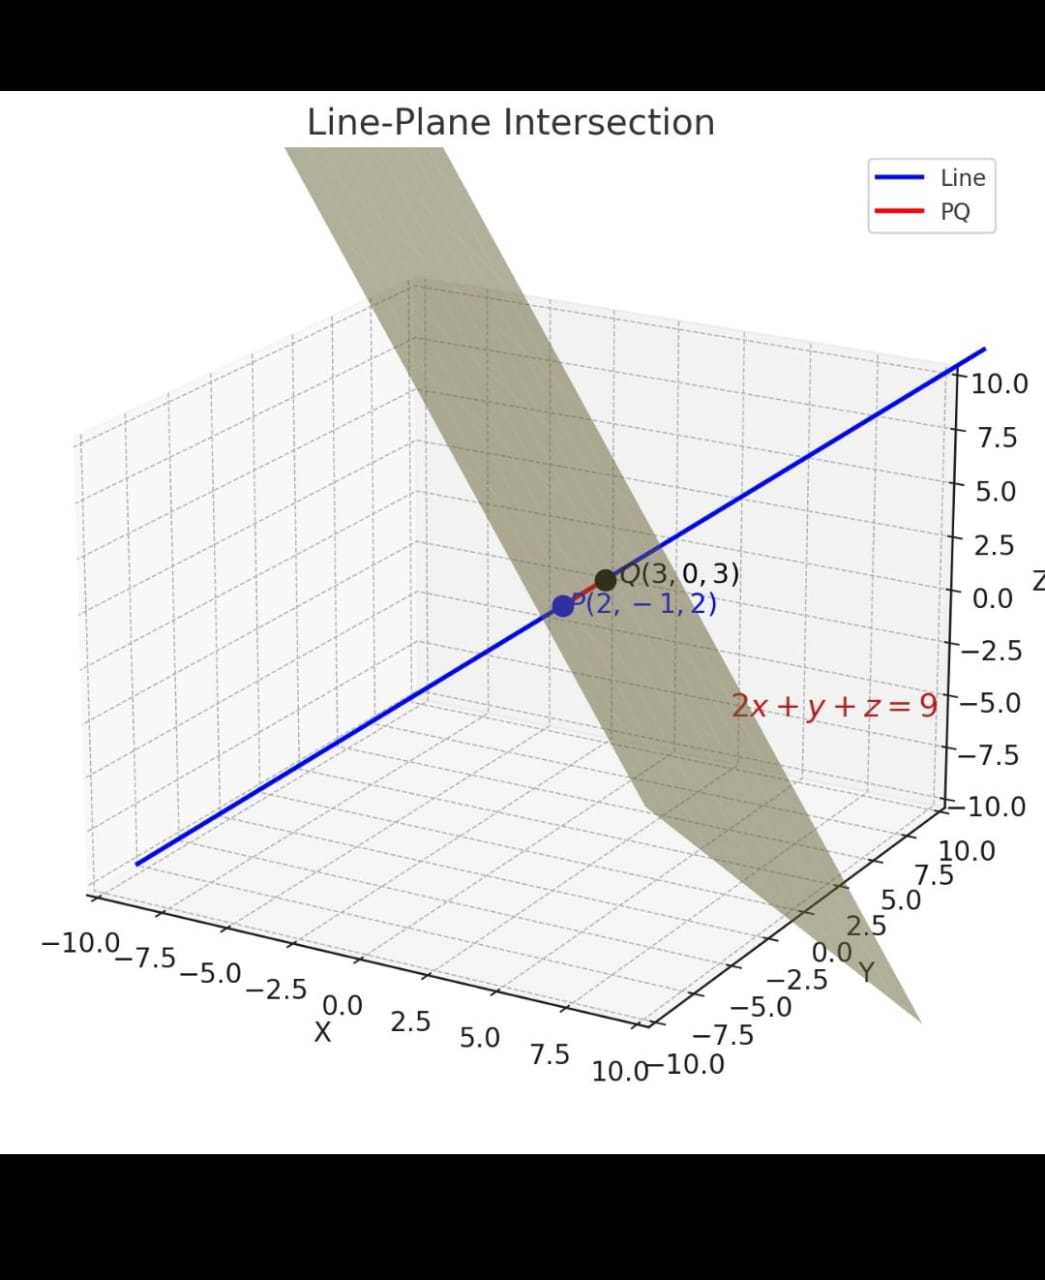
\includegraphics[width=0.65\textwidth]{matgeo-4.13.88.jpeg}
    \caption{}
    \label{fig:triangle5cm}
\end{figure}
\end{frame}

\end{document}
